\documentclass[11pt]{article}
\usepackage[a4paper,margin=24mm,top=21mm,bottom=22mm]{geometry}
\usepackage[T1]{fontenc}
\usepackage{lmodern,amsmath,amssymb,booktabs,graphicx,xcolor,hyperref}
\definecolor{ink}{HTML}{243847}
\definecolor{teal}{HTML}{087368}
\hypersetup{colorlinks=true,linkcolor=teal,urlcolor=teal,citecolor=teal,
 pdftitle={Clustered versus isolated target keys in QAOA pattern search},pdfauthor={Variational Quantum Algorithms project}}
\input{glyphtounicode}\pdfgentounicode=1
\newcommand{\LawRows}{%
Uniform start of one solid block & 8.97 & 121.00 \\
Uniform 16-element subset & 15.12 & 15.12 \\
Uniform 16-element subset with no neighbors & 15.17 & 14.24 \\
}
\newcommand{\ExactRows}{%
32 & 8 & 4.02 & 4.98 & 8.72 & 66.2 \\
16 & 16 & 8.03 & 8.97 & 16.00 & 65.5 \\
8 & 32 & 16.06 & 16.94 & 29.33 & 66.2 \\
}
\newcommand{\FeedbackRows}{%
One solid run & 8.78 & 15.15 & 41.59 & 7.84 & 14.91 & 9.45 \\
Four equal runs & 13.14 & 17.33 & 33.66 & 9.28 & 23.03 & 11.85 \\
Isolated & 14.61 & 15.97 & 31.67 & 10.11 & 23.76 & 12.97 \\
Uniform subset & 14.20 & 14.04 & 27.66 & 9.30 & 22.51 & 12.89 \\
Angle rectangle & 8.36 & 15.46 & 48.69 & 8.07 & 17.67 & 8.52 \\
}
\newcommand{\ArchiveRows}{%
Original sieve & 35.49 & 61.1 & 17.00 & 97.5 & 10.47 & 100.0 \\
Recursive sieve & 33.88 & 61.1 & 17.08 & 97.5 & 10.44 & 100.0 \\
Halton & 13.56 & 100.0 & 17.38 & 97.4 & 13.54 & 99.4 \\
Sobol & 29.22 & 63.9 & 16.98 & 97.5 & 13.31 & 100.0 \\
Random order & 17.51 & 97.0 & 17.28 & 97.5 & 17.17 & 97.3 \\
Pattern search & 26.10 & 68.1 & 30.54 & 62.0 & 37.13 & 48.3 \\
Recursive 13 + poll & 32.31 & 65.3 & 25.20 & 73.1 & 20.10 & 79.0 \\
Halton 13 + poll & 16.00 & 91.7 & 22.60 & 78.6 & 23.17 & 73.8 \\
Recursive bound + poll & 30.14 & 73.6 & 22.07 & 81.0 & 10.44 & 100.0 \\
Recursive patience & 29.89 & 65.3 & 28.09 & 67.0 & 30.17 & 60.6 \\
}
\newcommand{\EdgeRows}{%
8 & 16.94 & 32 & 16.94 & 32 & 27.33 & 153 \\
16 & 8.97 & 16 & 8.97 & 16 & 15.77 & 74 \\
32 & 4.98 & 8 & 4.98 & 8 & 8.22 & 57 \\
}

\newcommand{\VariableRows}{%
One variable-width block & 8.87 & 11.17 & 14.78 & 42.25 & 8.19 & 16.29 \\
Nearly equal blocks & 12.04 & 13.66 & 15.15 & 33.80 & 8.82 & 20.42 \\
Random unequal blocks & 11.54 & 12.64 & 14.70 & 35.34 & 8.70 & 19.97 \\
One dominant block & 9.79 & 11.62 & 15.02 & 39.74 & 8.63 & 17.61 \\
Guaranteed isolation & 14.45 & 13.46 & 13.96 & 26.65 & 9.22 & 20.44 \\
Uniform subset & 13.44 & 13.73 & 13.96 & 29.52 & 9.34 & 20.43 \\
}
\newcommand{\BoundRows}{%
One variable-width block & 20.0 & 100.0 & 100.0 & 100.0 & 100.0 & 84.3 \\
Nearly equal blocks & 6.8 & 85.5 & 85.0 & 85.0 & 99.7 & 79.2 \\
Random unequal blocks & 11.0 & 89.3 & 85.0 & 97.2 & 99.8 & 79.7 \\
One dominant block & 17.5 & 96.2 & 85.0 & 100.0 & 100.0 & 82.3 \\
Guaranteed isolation & 1.0 & 77.8 & 0.0 & 0.0 & 98.2 & 80.0 \\
Uniform subset & 1.9 & 78.3 & 0.0 & 1.5 & 98.8 & 79.5 \\
}
\newcommand{\HybridStageRows}{%
One variable-width block & 479 & 27 & 121 & 506 & 600 \\
Nearly equal blocks & 417 & 58 & 183 & 475 & 600 \\
Random unequal blocks & 426 & 52 & 174 & 478 & 600 \\
One dominant block & 468 & 26 & 132 & 494 & 600 \\
Guaranteed isolation & 372 & 108 & 228 & 480 & 600 \\
}

\setlength{\parindent}{0pt}
\setlength{\parskip}{5pt plus .6pt minus .4pt}
\setlength{\tabcolsep}{5pt}
\renewcommand{\arraystretch}{1.14}
\newcommand{\sect}[2]{\noindent{\sffamily\bfseries\large\color{ink}#1\hspace{.6em}#2}\par\smallskip}
\newcommand{\subt}[1]{\smallskip\noindent{\sffamily\bfseries\color{teal}#1}\par}
\newcommand{\capfig}[2]{{\small\textbf{Figure #1.} #2\par}}
\newcommand{\captab}[2]{{\small\textbf{Table #1.} #2\par}}
\newcommand{\E}{\mathbb E}
\pagestyle{myheadings}
\markboth{Target geometry and dyadic search}{\footnotesize\textsf{TARGET GEOMETRY AND DYADIC SEARCH}}
\begin{document}
\thispagestyle{plain}
{\sffamily\small\color{teal}\bfseries VARIATIONAL QUANTUM ALGORITHMS PROJECT}\par
\vspace{3pt}
{\sffamily\bfseries\fontsize{24}{27}\selectfont\color{ink}\raggedright Clustered versus isolated target keys in QAOA pattern search\par}
{\large A matched test of recursive-sieve initialization on the same MaxCut energies\par}
{\small Research draft prepared for Pauli Rikula \hfill 21 November 2026\par}
\vspace{2pt}{\color{teal}\rule{\linewidth}{1pt}}
\subt{Abstract}
Does clustering change whether a recursive sieve is a good starting method for QAOA pattern search? We compare two 13-call starts, recursive sieve and Halton sampling, followed by identical local polling under a 65-call budget. On 24 MaxCut graphs, all valid keys in the native encoding were isolated. The recursive-start hybrid hit 65.3\% of targets and the Halton-start hybrid hit 91.7\%. Placing the same valid energies in one consecutive block reversed their ranking. The recursive hybrid hit 79.0\% and the Halton hybrid 73.8\%. These are conditional results for two specified key layouts. We also test random subsets and blocks of unequal size, and measure how the information in a miss affects the local stage.

\sect{1}{What changes when the valid keys form a block?}
A key is valid if its QAOA energy meets the target threshold. In the native grid, no two valid integer keys were adjacent in any of the 72 graph/start cases \cite{hybrid}. For each case we kept all 256 energies, the starting energy and the threshold, and placed its valid energies in one block at a uniformly drawn legal position excluding the start. We used 32 placements per case. This changes the lookup order and the neighborhoods seen by local polling. The first 13 calls show the effect on initialization before either hybrid makes a local move.

\captab{1}{Share hitting the target (\%). Both hybrids use the same pattern search after call 13. The last column starts pattern search immediately. Native counts use 72 graph/start cases. The planted block uses 2,304 placements of those same cases.}
{\centering\small\begin{tabular}{@{}lrrrrr@{}}\toprule
& \multicolumn{2}{c}{By call 13, before handoff} & \multicolumn{3}{c}{By call 65, full optimizer}\\
Target keys & Recursive & Halton & Recursive start & Halton start & Immediate pattern\\\midrule
\InitializerRows\bottomrule\end{tabular}\par}

\textbf{Against Halton, clustering moved the recursive hybrid from 26.4 percentage points behind to 5.2 points ahead.} The paired change was 31.6 points (95\% graph-bootstrap interval 24.7 to 37.8). Section 8 describes the pairing. Uniformly isolated targets and single blocks also reversed the ranking in a separate binary-feedback test (Section 9). Section 6 counts first hits in each stage.

\begin{center}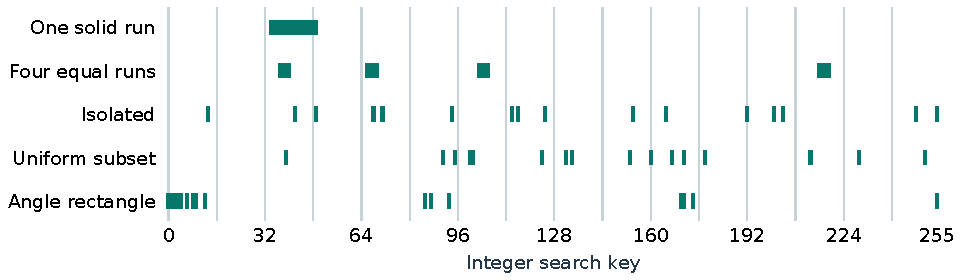
\includegraphics[width=.86\linewidth]{figures/geometry.pdf}\end{center}
\capfig{1}{Example target layouts with 16 valid keys among 256. Each tick marks a valid key. Gray lines mark the first 16 paid dyadic calls. A solid block means consecutive keys in the sieve's own integer order \cite{original}.}

\newpage
\sect{2}{The placement laws and the information in a miss}
The synthetic search grid has side $M=16$ or 32 and $N=M^2$ keys. We interleave the bits of the two angle indices, assigning the top bit to the first angle, as in the preceding joint-sieve implementation. For each grid we set $q=N/m$ to 8, 16 or 32. Each of the six size/density settings has 192 independent placement draws per law. Every method sees the same mask within a draw.

\captab{2}{Target laws conditional on $N$ and $m$. Valid runs are measured along the linear integer key order. Angle distance uses periodic boundaries on both axes.}
{\small\begin{tabular}{@{}p{.19\linewidth}p{.74\linewidth}@{}}\toprule
Law & How the valid points are drawn\\\midrule
One solid run & Draw $a$ uniformly from $0,\ldots,N-m$ and mark $a,\ldots,a+m-1$.\\
Four equal runs & Select uniformly among all configurations of four runs of length $m/4$, separated by at least one invalid key.\\
Isolated & Select uniformly among all $m$-subsets with \emph{no} adjacent keys.\\
Uniform subset & All $\binom Nm$ subsets have equal probability. Neighboring valid keys are allowed.\\
Angle rectangle & Choose a uniform toroidal translation of a rectangle of area $m$ and aspect ratio one or two. Choose its orientation with equal probability.\\\bottomrule
\end{tabular}}

For $r$ equal runs of length $\ell=m/r$, draw distinct sorted anchors $u_0<\cdots<u_{r-1}$ uniformly from $0,\ldots,N-m$. Start run $i$ at $u_i+i\ell$. Subtracting $i\ell$ recovers the anchors, giving a bijection with legal placements. In particular, a uniform subset has probability $1-\binom{N-m+1}{m}/\binom Nm$ of at least one adjacent pair. At $N=256,m=16$ this is 63.1\%. Random placement and guaranteed isolation answer different questions.

\subt{Exact consequences of assuming isolation}
For a paid query prefix $Q_t$, let $C_{i,j}$ count legal ways to place $j$ nonadjacent valid keys in the first $i$ keys while avoiding $Q_t$. Taking or skipping key $i-1$ gives
\[
  C_{i,j}=C_{i-1,j}+{\bf1}_{i-1\notin Q_t}\,C_{i-2,j-1},
  \qquad \Pr_{\rm isolated}(T>t)=C_{N,m}/\binom{N-m+1}{m}.
\]
The empty prefix has one empty placement. Summing the survival probabilities gives the exact mean for each fixed order. At $N=256,m=16$, the isolated law gives 15.17 calls for each dyadic order, 15.10 for Halton, and 14.24 for ascending keys. All three instead average 15.12 on a uniform unrestricted subset. For a uniformly placed solid block of the same size, the exact dyadic and ascending means are 8.97 and 121.00. These are results for standalone search orders.

\subt{What the optimizer observes}
The \emph{membership} objective is zero at every valid point and one elsewhere. The \emph{distance} objective returns the shortest four-neighbor distance to any valid point on the angle torus. Both have exactly the same zero set. Distance supplies informative objective values outside the target and is deliberately favorable to local search. Computing that table is part of constructing the simulated environment. An optimizer receives only requested values.

All 14 policies pay for the origin and have a 65-call ceiling. Pure original and recursive dyadic sieves use the same refinement levels. Halton and Sobol use the preceding study's two-dimensional schedules, and random search samples without replacement after the origin. Local pattern search polls in four directions and halves its step after an unsuccessful batch. The hybrids switch from the best paid pilot point after 13 or 33 calls, after four consecutive pilot calls without an improvement with cap 26, or at the model-implied deadline \cite{hybrid,torczon}. Local revisits count, and a converged local search may finish before the cap.

We report $\Pr(T\leq t)$ and mean capped time $L=\E[\min(T,66)]$ for the first valid evaluation $T$. An early-converged miss also scores 66. Full uncensored times are reported separately where all permutations were followed. No unconditional average over the five placement laws is used.

\newpage
\sect{3}{A deterministic deadline and two different means}
Let $d=2^{\lfloor\log_2\ell\rfloor}$, where $\ell\geq1$ is a credible lower bound on the length of at least one valid run. For $N$ a power of two, both deployed dyadic orders pay for key zero first. Their first $q_d=N/d$ keys are the set
\[
    \{0,d,2d,\ldots,N-d\}.
\]
The positive part of this prefix exhausts the dyadic levels whose entries are multiples of $d$. Any $d$ consecutive integer keys contain a multiple of $d$. Consequently $T\leq q_d$ \emph{for every placement} containing such a run. The argument requires no probability distribution. For four equal runs the guaranteed length is $m/4$. Substituting the total $m$ would assume a longer run than the model supplies.

For one nonwrapping run of power-of-two length $m\geq2$ with \emph{uniform start}, put $A=N-m+1$ and $q=N/m$. The original sieve with zero last has the expectation below, obtained by averaging its Lean-proved integer sum \cite{original}. Moving zero to call 1 changes the rank of the zero-start case from $q$ to 1 and delays every other first hit by one. Thus
\[
   \E T_{\rm canonical}=\frac{N(N-m+2)}{2mA},\qquad
   \E T_{\rm paid\ zero}=\E T_{\rm canonical}+1-\frac{q}{A}.
\]
Under the \emph{uniform $m$-subset law}, a fixed permutation independent of the labels instead has
\[
   \Pr(T>t)=\frac{\binom{N-t}{m}}{\binom Nm},\qquad
   \E T=\frac{N+1}{m+1}.
\]
Both identities follow by counting positions of the $m$ marked keys. For the mean, the $m+1$ exchangeable gaps share $N-m$ misses. For a \emph{solid} target with uniform start and a randomized search order \emph{after} paying for zero, the comparable mean is $1+(1-1/A)N/(m+1)$.

\captab{3}{Exact values for $N=256$. The three means use a uniformly placed block. The last column changes the target law to a uniform subset and gives the hit probability by $q$ for any fixed complete permutation.}
\begin{center}\small\begin{tabular}{@{}rrrrrr@{}}\toprule
$m$ & Deadline $q$ & Zero-last sieve & Paid-zero sieve & Paid-zero random & Uniform hit (\%)\\\midrule
\ExactRows\bottomrule
\end{tabular}\end{center}
\begin{center}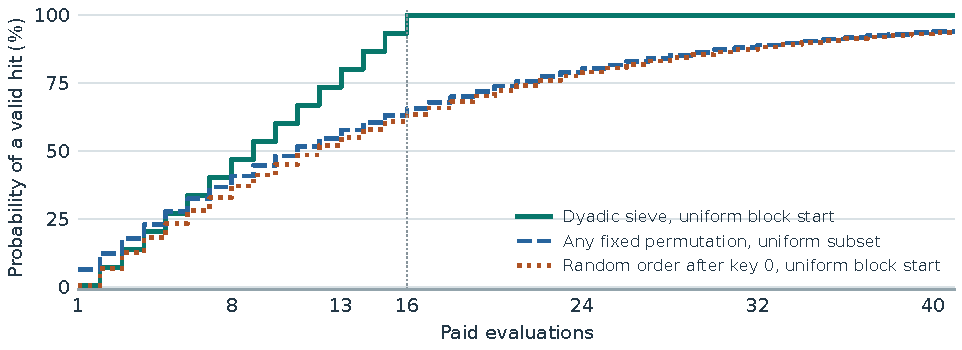
\includegraphics[width=.90\linewidth]{figures/exact_curves.pdf}\end{center}
\capfig{2}{Exact cumulative probabilities for $N=256,m=16$. Enumeration over all 15,142 placements at $N=64,256,1024,4096$ and $q=8,16,32$ verified the two solid-block means and the deadline for both dyadic implementations. The existing Lean theorem covers the original integer sum.}

\newpage
\sect{4}{Controlled masks and the cost of switching early}
On all 1,152 solid-block draws, both pure sieves hit by $q$, as the deterministic bound requires. Across the same six equally weighted size/density settings, the recursive sieve hit by $q$ on 66.0\% of uniform-subset draws and 64.8\% of guaranteed-isolated draws. The uniform-subset advantage over random order was 2.4 percentage points in this finite sample (paired 95\% interval $-1.6$ to $6.2$). The population difference is exactly zero under that law. On solid masks with membership feedback, waiting to $q$ instead of switching at 13 reduced mean capped time by 9.21 calls (8.31 to 10.12 fewer).

\begin{center}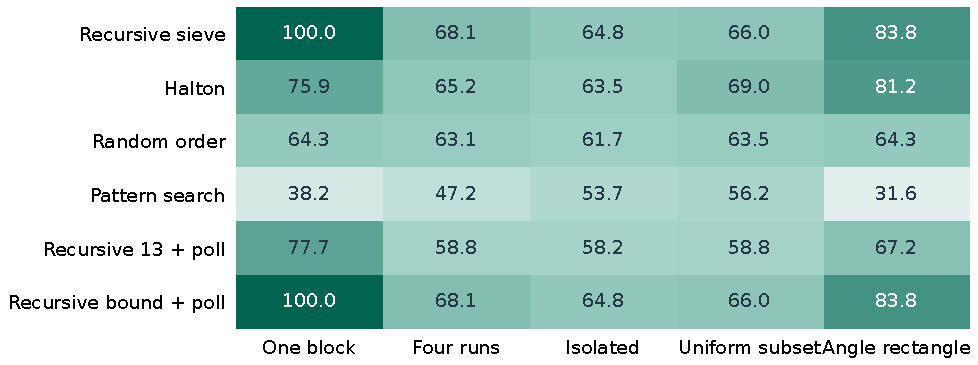
\includegraphics[width=.96\linewidth]{figures/conditional_hits.pdf}\end{center}
\capfig{3}{Hit by $q=N/m$ (\%) with membership feedback. Each column averages its own six prescribed settings equally. For the bound-based hybrid, $q$ is the pilot cap. Outside the solid-block column, using $m$ as a run-length assumption is deliberately tested under misspecification.}

\captab{4}{Mean capped calls at $N=256,m=16$ across 192 draws per row. Pure nonadaptive orders have the same first hits with either feedback. M denotes membership and D denotes exact angle distance. Lower is better.}
\begin{center}\small\begin{tabular}{@{}lrrrrrr@{}}\toprule
 & Recursive & Random & \multicolumn{2}{c}{Pattern search} & \multicolumn{2}{c}{Recursive 13 + poll}\\
Law & either & either & M & D & M & D\\\midrule
\FeedbackRows\bottomrule
\end{tabular}\end{center}

On the same solid targets at $N=256,m=16$, direct pattern search fell from 41.59 capped calls with a flat miss to 7.84 with distance feedback. This was slightly faster on average than the sampled recursive sieve (8.78), while the sieve retained its 16-call guarantee. The 8.97 in Table 3 is the exact mean across all 241 possible block locations. The 8.78 in Table 4 is a mean across 192 sampled starts. Geometry, miss information, and the choice of a mean or a deadline all affect the comparison.

An angle rectangle is another informative case. On the $16\times16$ grid with 16 valid cells, every sampled $4\times4$ rectangle met a dyadic prefix point by call 16. The prefix is a regular $4\times4$ angle lattice in this setting. Across the six tested size/density settings the corresponding rate is 83.8\%. The two-dimensional shape and its alignment with the query lattice matter independently of the longest one-dimensional run.

\newpage
\sect{5}{One unknown width, or several unequal solid blocks?}
For one block we enumerate every legal nonwrapping start at every integer width $m=8,\ldots,32$ for $N=256$ and $m=32,\ldots,128$ for $N=1024$. These yield 5,925 and 91,665 width/start pairs. Most widths are not powers of two. If width is uniform first and start is uniform conditional on width, the exact mean first-hit counts for either paid-zero sieve are 9.09 and 9.06. Choosing a width/start pair uniformly instead weights shorter widths more heavily. The corresponding means rise to 9.19 and 9.15. At $N=256$, increasing the width from 15 to 16 halves the worst case from 32 to 16, while the mean changes from 9.99 to 8.97.

\subt{A controlled generator for variable-size blocks}
For each grid size, the total number of valid keys $m$ is uniform on the same integer range. Independently, the number of planted blocks $r$ is uniform on $\{2,3,4,5\}$. We use six draws in every $(m,r)$ stratum. Each matched draw has three allocations:
\begin{itemize}\setlength{\itemsep}{0pt}
\item \textbf{Nearly equal.} Divide $m$ as evenly as possible. Randomly order the lengths that differ by one.
\item \textbf{Random unequal.} Choose $r-1$ distinct cuts uniformly in $1,\ldots,m-1$. Their spacings form an ordered positive composition. Redraw the all-equal case. At least two blocks have different lengths.
\item \textbf{One dominant.} One uniformly chosen block gets $m-r+1$ valid keys. Each of the others gets one.
\end{itemize}
The three allocations share identical empty gaps. Draw $r$ sorted anchors uniformly from $0,\ldots,N-m$, then set $a_i=u_i+\sum_{j<i}m_j$ for ordered lengths $m_j$. Adjacent blocks are separated by at least one invalid key. Each draw also has three count-matched controls: one variable-width interval, a uniform isolated set and a uniform unrestricted subset. All six layouts receive both objective signals. The primary variable-width grid has 600 draws per layout. The larger grid has 2,328. We report the two grids separately.

\begin{center}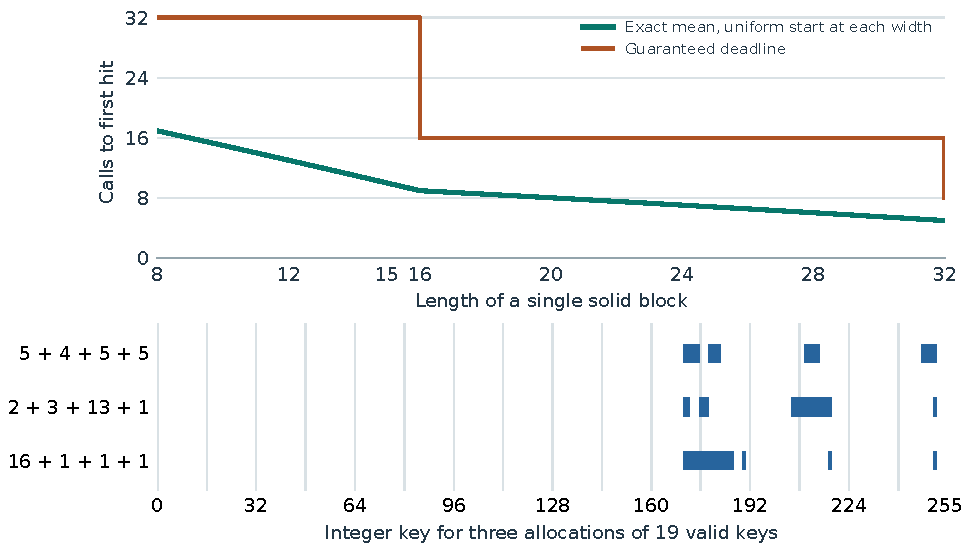
\includegraphics[width=.92\linewidth]{figures/variable_sizes.pdf}\end{center}
\capfig{4}{Above, exact first-hit mean and guaranteed deadline for every single-block width at $N=256$. Below, a recorded draw with $m=19,r=4$. The three allocations have identical gaps and total mass. Their largest blocks have lengths 5, 13 and 16. The corresponding longest-block deadlines are 64, 32 and 16 calls.}

\newpage
\sect{6}{What determines the handoff with unequal sizes?}
With $m$ valid keys in at most $r$ runs, the longest length satisfies $\ell_{\max}\geq\lceil m/r\rceil$. Writing $D(x)=N/2^{\lfloor\log_2 x\rfloor}$ gives $T\leq D(\ell_{\max})\leq D(\lceil m/r\rceil)$ for every placement. Using $D(m)$ can fail. In 16 keys, the blocks $\{1,2,3\}$ and $\{5\}$ escape the first four sieve queries $0,8,4,12$. Call 5 hits key 2. Our longest-block comparison receives the true length. In practice a known lower bound suffices.

\captab{5}{Mean capped calls over 600 cases per row at $N=256$, with uniform $m=8,\ldots,32$ and six draws per width and planned count. M denotes binary membership and D exact angle distance.}
{\centering\small\begin{tabular}{@{}lrrrrrr@{}}\toprule
 & Recursive & Halton & Random & \multicolumn{2}{c}{Pattern search} & Rec.\ 13 + poll\\
Size allocation & either & either & either & M & D & M\\\midrule
\VariableRows\bottomrule
\end{tabular}\par}

\captab{6}{Same cases with binary feedback. Rates are percentages. The $D(m)$ column gives the observed pure-sieve hit rate at that nominal deadline. The two certified columns use the run count or longest run.}
{\centering\small\begin{tabular}{@{}lrrrrrr@{}}\toprule
 & Mean & By & \multicolumn{2}{c}{Certified by 65} & \multicolumn{2}{c}{Observed by 65}\\
Allocation & $\ell_{\max}$ & $D(m)$ & count & longest & recursive & rec.\ 13\\\midrule
\BoundRows\bottomrule
\end{tabular}\par}

\captab{7}{First hits by stage in 600 paired cases per layout at $N=256$. The recursive sieve uses calls 1--13. Pattern search continues from its best point with up to 52 calls left. Each hit is credited to the stage that first found a valid key.}
{\centering\small\begin{tabular}{@{}lrrrrr@{}}\toprule
& Sieve & \multicolumn{2}{c}{Additional pattern hits} & \multicolumn{2}{c}{Combined by 65}\\
Block layout & 1--13 & Binary & Distance & Binary & Distance\\\midrule
\HybridStageRows\bottomrule
\end{tabular}\par}

On random unequal blocks, the sieve found 426 targets in 13 calls. Pattern search found 52 of the remaining 174 with binary feedback and all 174 with exact distance. Continuing the sieve reached 599 by call 65. With exact distance, immediate pattern search also reached all 600 and averaged 8.70 calls versus 10.78 for the hybrid. A solid block gives the sieve a coverage guarantee. The value of switching early depends on what a miss tells pattern search.

On these unequal blocks, 536 hit by $D(m)$. The count-based guarantee fit 65 calls in 510 cases, the longest-run guarantee in 583. At $N=1024$ the pure sieve hit all 2,328 unequal cases by 65 and the 13-call binary hybrid hit 79.6\%.

Holding total mass, count and gaps fixed, one dominant block saved 2.25 capped sieve calls over nearly equal blocks at $N=256$ (95\% bootstrap interval 1.51 to 3.02). Random unequal blocks saved 0.51 ($-0.20$ to 1.21). At $N=1024$ the savings were 3.73 and 1.27. Intervals resample the six paired draws within each width/count stratum.

\newpage
\sect{7}{A physical interval in a two-qubit QAOA circuit}
A one-edge MaxCut circuit provides a valid interval through its energy threshold. The depth-one QAOA state uses the negative cut Hamiltonian and the usual $X$ mixer \cite{farhi}. For a fixed mixer angle $\beta=\pi/8$, direct evaluation gives $E(\gamma)=-1/2+\sin(\gamma)/2$. Choose $N=256$, $c=a+(m-1)/2$ and the following angle and threshold:
\[
   \gamma_j=-\pi/2+2\pi(j-c)/N,\qquad
   \tau_m=-\frac{1+\cos(\pi m/N)}{2}.
\]
The statevector yields $E(\gamma_j)=-[1+\cos(2\pi(j-c)/N)]/2$. For $0\leq a\leq N-m$ the integer indices with $E\leq\tau_m$ are exactly $a,\ldots,a+m-1$. We verified this against the repository's simulator for every placement at $m=8,16,32$. Translating a precomputed energy cycle for each $a$ is exact by periodicity.

Use the same energies in three indexings. Physical keys take $j=k$. The odd-stride indexing takes $j=(1+N/2)k\bmod N$. This is a bijection, fixes each even key, and separates consecutive indices so far in physical angle that the chosen $m$ valid keys become isolated. A third indexing draws a uniform random permutation independently for each $(m,a)$. No energies or target counts change.

\begin{center}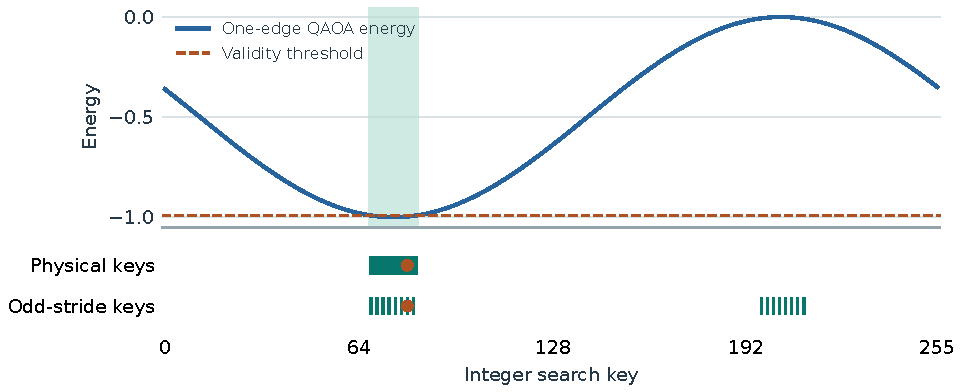
\includegraphics[width=.94\linewidth]{figures/one_edge.pdf}\end{center}
\capfig{5}{One physical interval at $a=68,m=16$. The orange dots indicate the same first valid query in both indexings. Although the lower valid set has 16 isolated keys, the early even-key queries are preserved.}
\captab{8}{Uncensored recursive first-hit ranks over all equally weighted block starts. Shuffled values use one seeded permutation per placement. Max is empirical for the shuffled column.}
\begin{center}\small\begin{tabular}{@{}rrrrrrr@{}}\toprule
 & \multicolumn{2}{c}{Physical interval} & \multicolumn{2}{c}{Isolated, odd stride} & \multicolumn{2}{c}{Shuffled}\\
$m$ & Mean & Max & Mean & Max & Mean & Max\\\midrule
\EdgeRows\bottomrule
\end{tabular}\end{center}

All 715 odd-stride cases had exactly the same first-hit rank as their physical counterparts for each sieve. Before the solid interval's deadline every divisor-$m$ prefix key is even and is fixed by this encoding. This example establishes the logical boundary of the result: a solid interval is sufficient for the deadline. A scattered set can also be found reliably when the encoding preserves the early queries that intersect it.

\newpage
\sect{8}{Reindexing the earlier MaxCut energies}
The 24 confirmation graphs came from six strata ($n=7,8,9$ vertices and edge probability 0.35 or 0.60, conditioned on connectedness). We used the same three starts per graph, $16\times16$ exact statevector energies and archived threshold $E_0-0.8(E_0-E_{\min})$ \cite{hybrid}. Relative key zero is the common, invalid start. The 72 target counts were 8 for 17 cases, 16 for 38, 24 for 12, and 32 for five.

For each case we paired 32 seeded reindexings. The \emph{solid} layout places its $m$ valid energies in one block with start uniform on $1,\ldots,N-m$. The \emph{shuffled} layout assigns them to a uniform $m$-subset of keys $1,\ldots,N-1$. Each graph, start and draw receives equal weight within its level. Both layouts keep key zero's energy, threshold and entire energy multiset. The same two shuffled lists assign valid and invalid energies in key order under both treatments. Native indexing retains the physical circuit-angle map. The relabelings are controlled lookup-table experiments designed to test geometry. Constructing them requires offline knowledge of which points are valid.

\captab{9}{Means on these 24 graphs, three starts and 32 paired draws per start. $L$ is capped first-hit time. H is the percentage meeting the energy target by 65 calls. Repeated native traces count once in the graph-level weighting.}
\begin{center}\small\begin{tabular}{@{}lrrrrrr@{}}\toprule
 & \multicolumn{2}{c}{Native} & \multicolumn{2}{c}{Shuffled} & \multicolumn{2}{c}{One solid block}\\
Method & $L$ & H & $L$ & H & $L$ & H\\\midrule
\ArchiveRows\bottomrule
\end{tabular}\end{center}
\begin{center}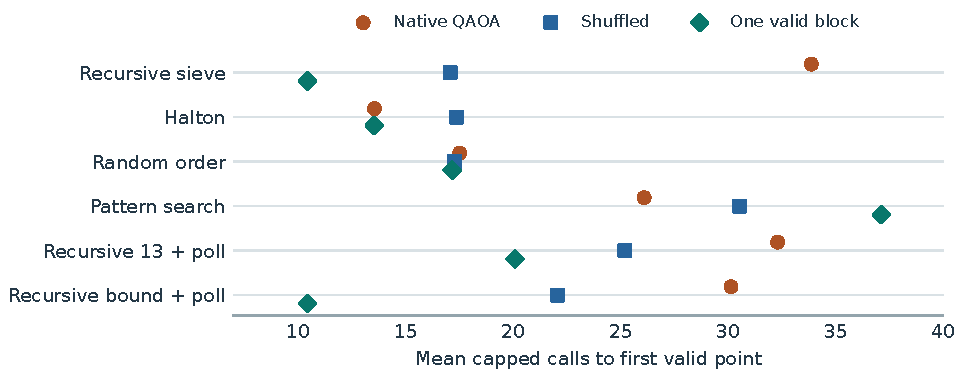
\includegraphics[width=.90\linewidth]{figures/matched_qaoa.pdf}\end{center}
\capfig{6}{Same graph energies under three indexings. The move from native to solid reduced recursive mean capped time by 23.44 calls (paired graph-bootstrap 95\% interval 21.75 to 25.31 fewer). Solid versus shuffled saved 6.64 calls (6.06 to 7.24).}

For Table 1, we compute the recursive-start minus Halton-start hit rate within each graph and layout, averaging the three starts and the placements for each start. We subtract the native difference from the solid-block difference and resample whole paired graphs 10,000 times within the six graph strata. Against immediate pattern search the corresponding change at call 65 was 33.6 percentage points (95\% interval 29.7 to 37.7). Pure recursive sampling hit all 2,304 solid placements within its guaranteed deadline, and 44 of 72 native cases by call 65.

\newpage
\sect{9}{When is the initial sieve worth its calls?}
On the native MaxCut grids, immediate pattern search reached 68.1\% and the recursive-start hybrid 65.3\%. On the planted blocks, giving the same pattern search a recursive start raised coverage from 48.3\% to 79.0\%. Halton was the stronger initializer on the native isolated keys (Table 1).

Under binary feedback with 8--32 valid keys in 256, the same 13-call-start comparison gave 506/600 hits for recursive versus 468/600 for Halton on single blocks, and 480/600 versus 518/600 on uniformly isolated keys. On random unequal blocks it gave 478/600 versus 483/600. A single intact block and several unequal blocks can favor different starts even at the same target count.
A known run of at least $\ell$ keys guarantees a first sieve hit by $N/2^{\lfloor\log_2\ell\rfloor}$ calls. Stop on a hit. An earlier switch trades that coverage for local progress. The 13-call and 33-call splits are choices to evaluate against the feedback and placement law of the intended workload.

For the separate comparison of \emph{pure} search orders in Figure 7, let $\pi$ be the probability of the solid reindexing of Section 8, with the native law otherwise. The expected capped loss of policy $j$ is $L_j(\pi)=(1-\pi)L_{j,\mathrm{native}}+\pi L_{j,\mathrm{solid}}$. Relative to Halton, the recursive sieve cost 20.32 more calls on native inputs and saved 3.10 on solid reindexings. This gives a crossover at $\pi=20.32/(20.32+3.10)=86.8\%$ (graph-bootstrap interval 84.9--88.7\%). The prevalence of either geometry on a future workload is unknown.

\begin{center}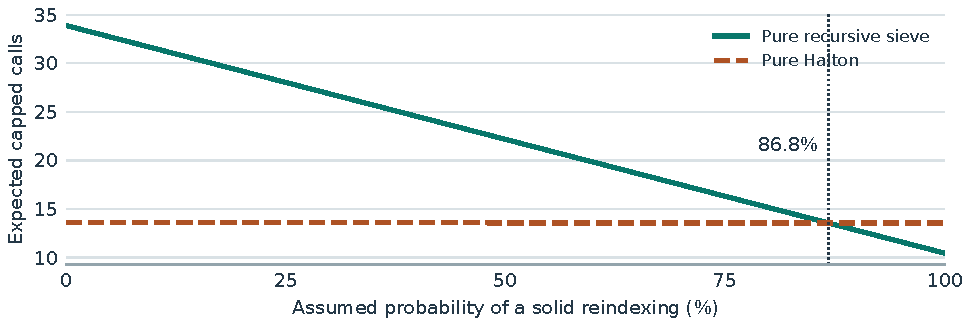
\includegraphics[width=.81\linewidth]{figures/mixture.pdf}\end{center}
\capfig{7}{Expected capped loss as the assumed mixture changes. Under these measured conditional losses, pure recursive sampling has the smaller mean to the right of the crossing. Altering the target law, the metadata given to a solver, or the cost assigned to a miss changes the comparison.}

\subt{Reproduction and scope}
The companion directory contains the first-hit ranks and full costs of 820,224 budgeted policy runs, exact counts, all 2,145 one-edge records, and reconstruction scripts. Synthetic intervals resample paired draws within design strata. Archived intervals resample whole graphs after averaging starts and remaps within each graph. Each interval uses 10,000 draws. The experiments measure noiseless classical queries. Hardware costs and the prevalence of each geometry require independent data.

\begingroup\footnotesize
\renewcommand{\refname}{\sffamily\small\color{teal}References}
\begin{thebibliography}{9}\setlength{\itemsep}{0pt}\setlength{\parskip}{0pt}
\bibitem{original} P. Rikula. \emph{Coarse-to-Fine Dyadic Sampling: An Exact First-Hit Result and an Exploratory QAOA Benchmark}. Zenodo, 2026. \href{https://doi.org/10.5281/zenodo.24382960}{DOI 10.5281/zenodo.24382960}. \href{https://github.com/kummahiih/variational-quantum-algorithms/tree/0ab4abc6ea3a980cd86ac77447979b5e469b54d5/paper}{Manuscript and data}.
\bibitem{hybrid} Variational Quantum Algorithms project. \emph{Initializing QAOA pattern search on nonclustered target keys}. 2026. \href{https://github.com/kummahiih/variational-quantum-algorithms/blob/main/paper/hybrid/hybrid_qaoa.pdf}{Revised paper}. \href{https://github.com/kummahiih/variational-quantum-algorithms/tree/8b066ec58925dd05dda6712aa5943c4f8b4d4487/paper/hybrid}{Research draft, engine and graph records}.
\bibitem{torczon} V. Torczon. On the convergence of pattern search algorithms. 1997. \href{https://doi.org/10.1137/S1052623493250780}{SIAM J. Optim. 7, 1--25}.
\bibitem{farhi} E. Farhi, J. Goldstone and S. Gutmann. A Quantum Approximate Optimization Algorithm. 2014. \href{https://arxiv.org/abs/1411.4028}{arXiv:1411.4028}.
\end{thebibliography}
\endgroup
{\footnotesize\textbf{Declaration of generative AI assistance.} OpenAI Codex implemented the simulation, ran the checks and drafted this manuscript at the project owner's request. This draft awaits author review.\par}
\end{document}
